\section{Diagrama de Entidade-Relacionamento}

\hspace{0.5cm} Os modelos de dados representam a estrutura das informações que serão armazenadas e manipuladas pelo sistema.
Eles definem as entidades, seus atributos e os relacionamentos entre elas, garantindo a integridade e a consistência dos dados.

Na \ref{fig:der}, estão descritos as entidades principais do sistema em DER e suas respectivas descrições.

\begin{figure}[h]
    \centering
    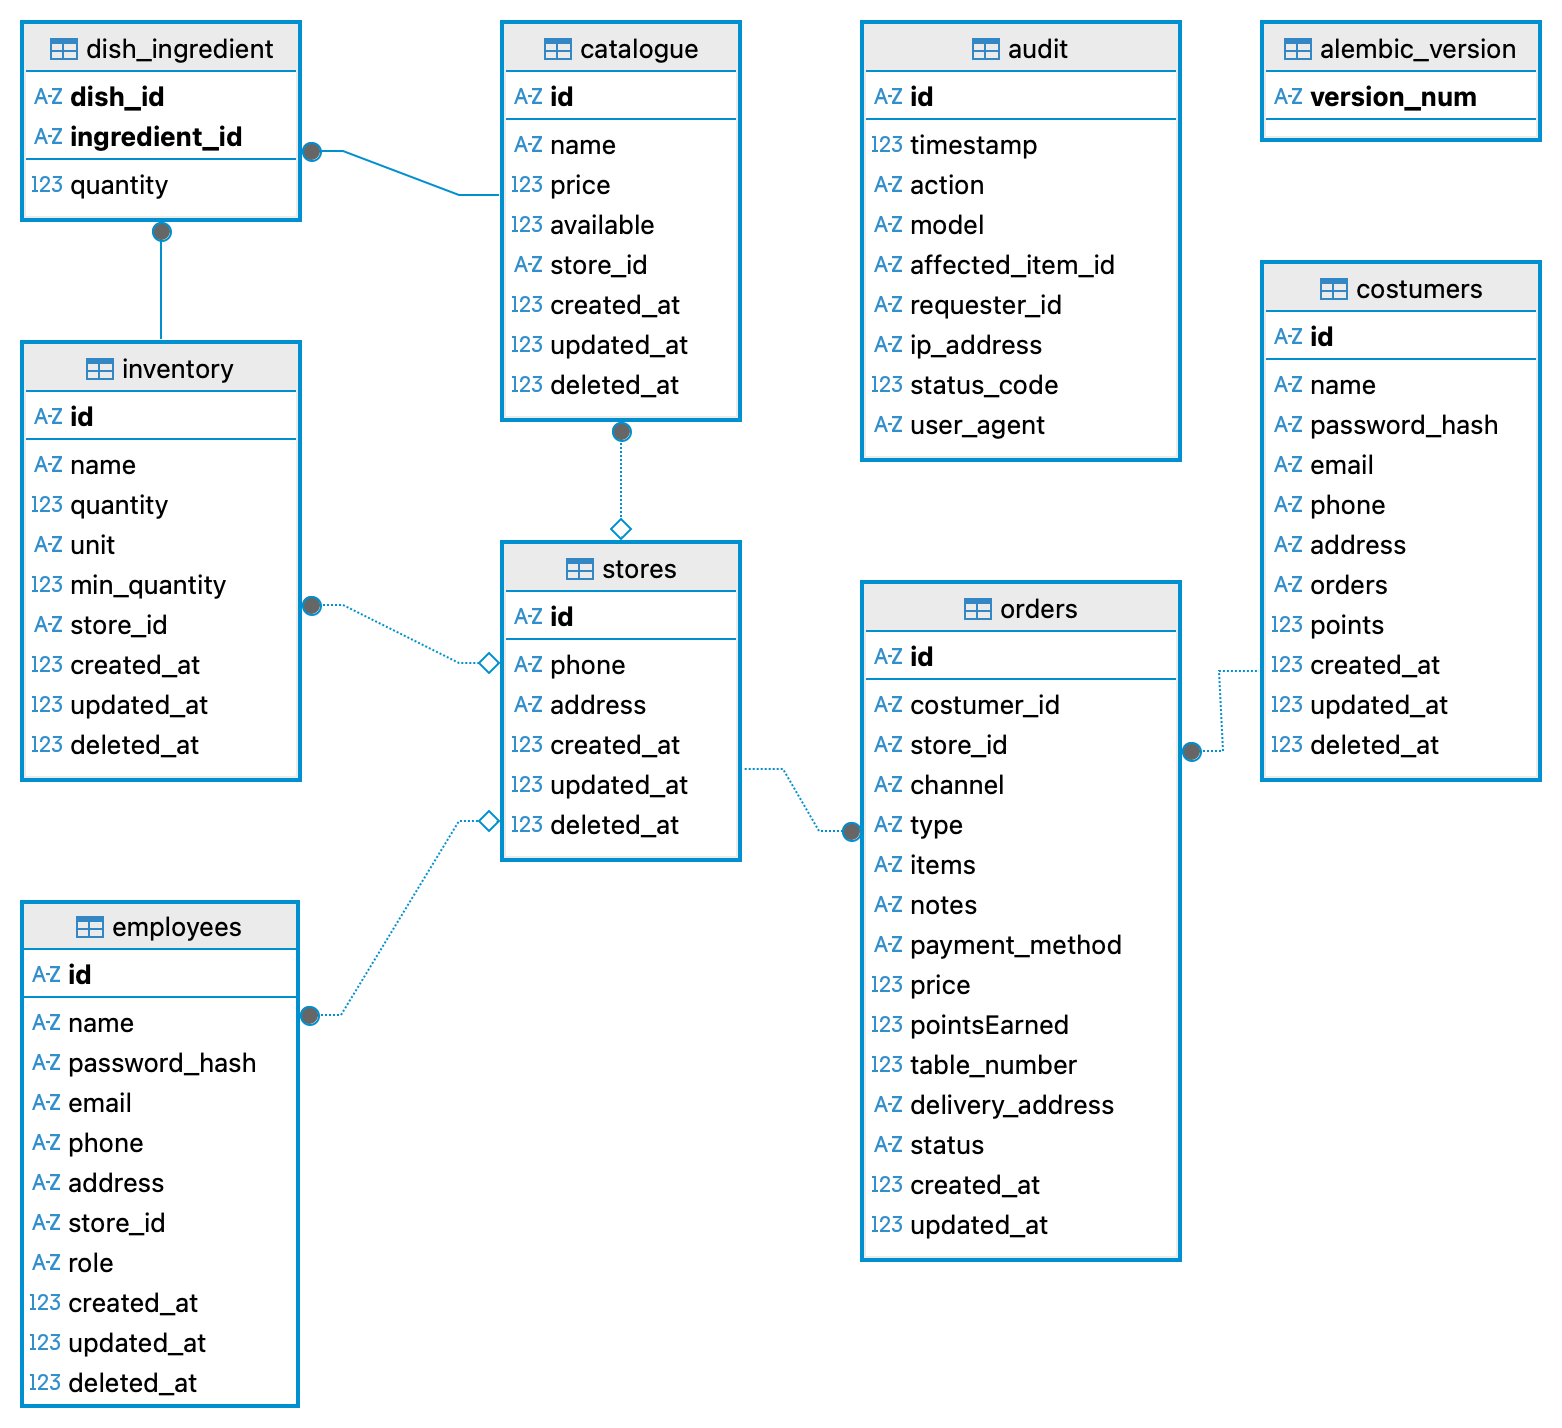
\includegraphics[width=\textwidth]{images/food_service.png}
    \caption{DER do Raízes do Nordeste}
    \label{fig:der}
\end{figure}
